% !TEX TS-program = xelatex
% !BIB program = biber
% !TEX encoding = UTF-8 Unicode

\documentclass[
  twoside,
  openright,
  degree    = master,               % degree = master | doctor
  language  = english,              % language = chinese | english
  fontset   = default,              % fontset = default | template | system | overleaf
                                    %   default  自由授權替代字型，Overleaf 與本機皆可用
                                    %   template 使用者自行放進 fonts/ 的字型（見 fonts/README.md）
                                    %   system   由作業系統解析字族名稱
                                    %   overleaf Overleaf 影像內建字型
  mathfont  = stix,                 % mathfont = default | termes | stix
  watermark = true,                 % watermark = true | false
  doi       = true,                 % doi = true | false
]{ntuthesis}

% !TeX root = ./main.tex

% --------------------------------------------------
% 資訊設定（Information Configs）
% --------------------------------------------------
%
% 這個檔案只放個人資料，版面與樣式設定一律寫在 main.tex。
% 星號版本（university* 等）是英文，無星號版本是中文。
%
% This file holds personal information only; style and layout live in main.tex.
% The starred keys hold the English text, the unstarred ones the Chinese.

\ntusetup{
  university*   = {National Taiwan University},
  university    = {國立臺灣大學},
  college       = {工學院},
  college*      = {College of Engineering},
  institute     = {工業工程學研究所},
  institute*    = {Institute of Industrial Engineering},
  title         = {論文標題},
  title*        = {Title of the Thesis},
  author        = {史迪奇},
  author*       = {Stitch},
  ID            = {R12345678},
  advisor       = {莉蘿},
  advisor*      = {Lilo},
% date          = {2026-08-11},         % 若註解掉，則預設為當天
% oral-date     = {2026-01-19},         % 若註解掉，則預設為當天
  DOI           = {DOI Number},         % 送出論文後由臺大配發
  keywords      = {關鍵字一, 關鍵字二, 關鍵字三},
  keywords*     = {Keyword One, Keyword Two, Keyword Three},
  email         = {stitch@ntu.edu.tw},  % 以下兩項不會排進論文，
  ORCID         = {0000-0000-0000-0000},% 只供 generate_tdr_upload_script.py 使用
}

% --------------------------------------------------
% 口試委員名單（Oral Examination Committee）
% --------------------------------------------------
%
% 這份名單不會排進論文。審定書上的簽名由委員親筆簽署，模板不代排；名單只給
% generate_tdr_upload_script.py 讀取，用來填寫 TDR 上傳表單。
%
% 每位委員呼叫一次 \ntucommittee，順序即為表單上的順序。欄位：
%
%   name    委員中文姓名
%   name*   委員英文姓名
%   email   聯絡信箱
%   title   身分：指導教授、共同指導教授、口試委員
%   ORCID   選填
%
% This list is never typeset. Signatures on the letter are handwritten; the list
% exists only for generate_tdr_upload_script.py to fill in the TDR form. Call
% \ntucommittee once per member, in the order they should appear. ORCID is
% optional; every other field is required.

\ntucommittee{
  name   = {莉蘿},
  name*  = {Lilo},
  email  = {lilo@ntu.edu.tw},
  title  = {指導教授},
  ORCID  = {0000-0000-0000-0001},
}

\ntucommittee{
  name   = {奶奶},
  name*  = {Nani},
  email  = {nani@ntu.edu.tw},
  title  = {共同指導教授},
}

\ntucommittee{
  name   = {金剛},
  name*  = {Jumba},
  email  = {jumba@example.edu.tw},
  title  = {口試委員},
  ORCID  = {0000-0000-0000-0002},
}

\ntucommittee{
  name   = {普里克利},
  name*  = {Pleakley},
  email  = {pleakley@example.edu.tw},
  title  = {口試委員},
}

% wherelist:
%   A compact IEEE-like "where" list for explaining symbols after an equation.
%   The word "where" is printed automatically.
%
% Usage:
%
%   \begin{equation}
%   ...
%   \end{equation}
%   \begin{wherelist}
%     \item[$p_i$] is the error rate of the i-th error position;
%     \item[$e_i$] is 1 if the i-th error occurred and 0 otherwise.
%   \end{wherelist}
%
% Optional arguments:
%
%   \begin{wherelist}[<left indent>][<gap between label and explanation>]
%
% Defaults:
%
%   \begin{wherelist}              % equivalent to [\parindent][1em]
%   \begin{wherelist}[1em]         % equivalent to [1em][1em]
%   \begin{wherelist}[1em][0.75em] % custom indent and custom label gap
%
\NewDocumentEnvironment{wherelist}{O{\parindent} O{1em} +b}{%
  \begingroup

  % Local spacing settings.
  %
  % This tightens the space between the preceding displayed equation and
  % the printed word "where". Make this less negative if the gap is too tight,
  % or more negative if the gap is still too large.
  \def\wherelistEquationToWhereCorrection{-0.45\baselineskip}%

  % This removes the extra paragraph/list gap between "where" and the items.
  \def\wherelistWhereToItemsCorrection{-\parskip}%

  % Local readable aliases for TeX scratch dimensions.
  \dimendef\wherelistLabelWidth=0
  \dimendef\wherelistCandidateWidth=2

  \wherelistLabelWidth=0pt
  \wherelistCandidateWidth=0pt

  % First pass: measure the widest optional label in \item[...].
  {%
    \RenewDocumentCommand{\item}{o}{%
      \IfNoValueTF{##1}{%
        \wherelistCandidateWidth=0pt
      }{%
        \settowidth{\wherelistCandidateWidth}{##1}%
      }%
      \ifdim\wherelistCandidateWidth>\wherelistLabelWidth
        \global\wherelistLabelWidth=\wherelistCandidateWidth
      \fi
      \ignorespaces
    }%
    \setbox0=\vbox{%
      \hsize=\maxdimen
      \parindent=0pt
      #3%
    }%
  }%

  \par
  \nopagebreak[4]%
  \vspace{\wherelistEquationToWhereCorrection}%
  \nopagebreak[4]%
  \noindent where%
  \par\nobreak
  \vspace{\wherelistWhereToItemsCorrection}%
  \nopagebreak[4]%

  % Second pass: typeset the real list using the measured label width.
  \begin{list}{}{%
    \setlength{\labelwidth}{\wherelistLabelWidth}%
    \setlength{\labelsep}{#2}%
    \setlength{\leftmargin}{\dimexpr #1 + \wherelistLabelWidth + #2\relax}%
    \setlength{\itemindent}{0pt}%
    \setlength{\listparindent}{0pt}%
    \setlength{\parsep}{0pt}%
    \setlength{\itemsep}{0pt}%
    \setlength{\topsep}{0pt}%
    \setlength{\partopsep}{0pt}%
    \setlength{\rightmargin}{0pt}%
    \renewcommand{\makelabel}[1]{##1\hfil}%
  }%
  #3%
  \end{list}%

  \endgroup
  \par
  \csname @endpetrue\endcsname
  \ignorespacesafterend
}{}
\addbibresource{back/references.bib}

\newcommand{\showcoverseal}{}        % Required for submission; comment out only to hide the cover watermark in drafts.

\begin{document}

% 封面與口試審定
% Cover and Verification Letter
\makecover                          % 論文封面（Cover）
\makeverification                   % 口試委員審定書（Verification Letter）

% 致謝與論文摘要
% Acknowledgement and Abstract
% !TeX root = ../main.tex

% 臺大格式規範：序言或謝辭依個人意願自行決定是否撰寫，須另頁書寫，
% 內容力求簡單扼要，以不超過一頁為原則。不寫的話，把 main.tex 裡
% % !TeX root = ../main.tex

% 臺大格式規範：序言或謝辭依個人意願自行決定是否撰寫，須另頁書寫，
% 內容力求簡單扼要，以不超過一頁為原則。不寫的話，把 main.tex 裡
% % !TeX root = ../main.tex

% 臺大格式規範：序言或謝辭依個人意願自行決定是否撰寫，須另頁書寫，
% 內容力求簡單扼要，以不超過一頁為原則。不寫的話，把 main.tex 裡
% \input{front/acknowledgement} 那一行註解掉即可。
%
% NTU rules: optional, starts on its own page, one page at most. To leave it
% out, comment out the \input{front/acknowledgement} line in main.tex.

\begin{acknowledgement}

在這裡感謝指導教授、口試委員、實驗室夥伴、經費或計算資源的提供者，以及家人朋友。
刪掉這段文字，換成自己的謝辭。

若論文寫作過程中使用了生成式 AI 工具，許多系所要求在此揭露使用範圍。

\end{acknowledgement}
 那一行註解掉即可。
%
% NTU rules: optional, starts on its own page, one page at most. To leave it
% out, comment out the % !TeX root = ../main.tex

% 臺大格式規範：序言或謝辭依個人意願自行決定是否撰寫，須另頁書寫，
% 內容力求簡單扼要，以不超過一頁為原則。不寫的話，把 main.tex 裡
% \input{front/acknowledgement} 那一行註解掉即可。
%
% NTU rules: optional, starts on its own page, one page at most. To leave it
% out, comment out the \input{front/acknowledgement} line in main.tex.

\begin{acknowledgement}

在這裡感謝指導教授、口試委員、實驗室夥伴、經費或計算資源的提供者，以及家人朋友。
刪掉這段文字，換成自己的謝辭。

若論文寫作過程中使用了生成式 AI 工具，許多系所要求在此揭露使用範圍。

\end{acknowledgement}
 line in main.tex.

\begin{acknowledgement}

在這裡感謝指導教授、口試委員、實驗室夥伴、經費或計算資源的提供者，以及家人朋友。
刪掉這段文字，換成自己的謝辭。

若論文寫作過程中使用了生成式 AI 工具，許多系所要求在此揭露使用範圍。

\end{acknowledgement}
 那一行註解掉即可。
%
% NTU rules: optional, starts on its own page, one page at most. To leave it
% out, comment out the % !TeX root = ../main.tex

% 臺大格式規範：序言或謝辭依個人意願自行決定是否撰寫，須另頁書寫，
% 內容力求簡單扼要，以不超過一頁為原則。不寫的話，把 main.tex 裡
% % !TeX root = ../main.tex

% 臺大格式規範：序言或謝辭依個人意願自行決定是否撰寫，須另頁書寫，
% 內容力求簡單扼要，以不超過一頁為原則。不寫的話，把 main.tex 裡
% \input{front/acknowledgement} 那一行註解掉即可。
%
% NTU rules: optional, starts on its own page, one page at most. To leave it
% out, comment out the \input{front/acknowledgement} line in main.tex.

\begin{acknowledgement}

在這裡感謝指導教授、口試委員、實驗室夥伴、經費或計算資源的提供者，以及家人朋友。
刪掉這段文字，換成自己的謝辭。

若論文寫作過程中使用了生成式 AI 工具，許多系所要求在此揭露使用範圍。

\end{acknowledgement}
 那一行註解掉即可。
%
% NTU rules: optional, starts on its own page, one page at most. To leave it
% out, comment out the % !TeX root = ../main.tex

% 臺大格式規範：序言或謝辭依個人意願自行決定是否撰寫，須另頁書寫，
% 內容力求簡單扼要，以不超過一頁為原則。不寫的話，把 main.tex 裡
% \input{front/acknowledgement} 那一行註解掉即可。
%
% NTU rules: optional, starts on its own page, one page at most. To leave it
% out, comment out the \input{front/acknowledgement} line in main.tex.

\begin{acknowledgement}

在這裡感謝指導教授、口試委員、實驗室夥伴、經費或計算資源的提供者，以及家人朋友。
刪掉這段文字，換成自己的謝辭。

若論文寫作過程中使用了生成式 AI 工具，許多系所要求在此揭露使用範圍。

\end{acknowledgement}
 line in main.tex.

\begin{acknowledgement}

在這裡感謝指導教授、口試委員、實驗室夥伴、經費或計算資源的提供者，以及家人朋友。
刪掉這段文字，換成自己的謝辭。

若論文寫作過程中使用了生成式 AI 工具，許多系所要求在此揭露使用範圍。

\end{acknowledgement}
 line in main.tex.

\begin{acknowledgement}

在這裡感謝指導教授、口試委員、實驗室夥伴、經費或計算資源的提供者，以及家人朋友。
刪掉這段文字，換成自己的謝辭。

若論文寫作過程中使用了生成式 AI 工具，許多系所要求在此揭露使用範圍。

\end{acknowledgement}
         % 致謝（Acknowledgement）
% !TeX root = ../main.tex

% 臺大格式規範：中英文摘要各以不超過三頁為原則，內容應包含論述重點、方法或程序、
% 結果與討論及結論。經系所同意以英文撰寫論文者，仍須附中文摘要。
% 關鍵字不必寫在這裡，改在 ntusetup.tex 的 keywords / keywords* 設定，
% 排版時會自動附在摘要末尾。
%
% NTU rules: three pages maximum each. State the problem, the method, the
% results, and the conclusion. A thesis written in English still needs the
% Chinese abstract. Keywords are NOT typed here; set them in ntusetup.tex and
% the class appends them automatically.

\begin{abstract}

在這裡寫中文摘要。刪掉這段文字，換成論述重點、方法或程序、結果與討論及結論。

\zhlipsum[1][name=trad]

\end{abstract}

\begin{abstract*}

Write the English abstract here. Replace this paragraph with the problem, the
method, the results, and the conclusion.

\setlipsum{language=english}
\lipsum[1]

\end{abstract*}
              % 摘要（Abstract）

% 生成目錄與符號列表
% Contents of Tables and Denotation
\maketableofcontents                % 目錄（Table of Contents）
\makelistoffigures                  % 圖目錄（List of Figures）
\makelistoftables                   % 表目錄（List of Tables）
% !TeX root = ../main.tex

% 符號列表。中括號裡是符號，大括號裡是說明。
% 下面每個類別各放一個例子，涵蓋數學符號、排版符號與英文縮寫三種標籤，
% 三者的排版方式相同。請留下與自己領域相關的幾項，其餘刪除；
% 整章不需要的話，把 main.tex 裡 % !TeX root = ../main.tex

% 符號列表。中括號裡是符號，大括號裡是說明。
% 下面每個類別各放一個例子，涵蓋數學符號、排版符號與英文縮寫三種標籤，
% 三者的排版方式相同。請留下與自己領域相關的幾項，其餘刪除；
% 整章不需要的話，把 main.tex 裡 % !TeX root = ../main.tex

% 符號列表。中括號裡是符號，大括號裡是說明。
% 下面每個類別各放一個例子，涵蓋數學符號、排版符號與英文縮寫三種標籤，
% 三者的排版方式相同。請留下與自己領域相關的幾項，其餘刪除；
% 整章不需要的話，把 main.tex 裡 \input{front/denotation} 那一行註解掉。
%
% 選用參數 [3cm] 是標籤欄寬度，預設 2.5cm。標籤比欄寬長時說明會被推開，
% 把數字調大即可。
%
% One example per broad field, covering the three kinds of label this
% environment handles: maths, typographic marks, and plain abbreviations. Keep
% the ones that fit your discipline and delete the rest. The optional [3cm] is
% the label column width; widen it if a label overruns.

\begin{denotation}[3cm]

% 1. 人文與文化 Humanities and culture
\item[$\dagger$]{
  obelus, marking a corrupt or doubtful passage in a critical edition
}

% 2. 社會、政治與公共政策 Social science, politics, and public policy
\item[GDP]{
  gross domestic product
}

% 3. 法律與制度 Law and institutions
\item[\S]{
  section sign, citing an article of a statute
}

% 4. 商業與管理 Business and management
\item[ROI]{
  return on investment
}

% 5. 基礎科學與數學 Basic science and mathematics
\item[$\hbar$]{
  reduced Planck constant
}

% 6. 工程、資訊與科技 Engineering, computing, and technology
\item[$O(\cdot)$]{
  asymptotic upper bound on a function's growth rate
}

% 7. 生物、農業與環境 Life science, agriculture, and environment
\item[$\mathrm{LD}_{50}$]{
  median lethal dose, the dose fatal to half of a test population
}

% 8. 醫學、健康與公衛 Medicine, health, and public health
\item[OR]{
  odds ratio
}

\end{denotation}
 那一行註解掉。
%
% 選用參數 [3cm] 是標籤欄寬度，預設 2.5cm。標籤比欄寬長時說明會被推開，
% 把數字調大即可。
%
% One example per broad field, covering the three kinds of label this
% environment handles: maths, typographic marks, and plain abbreviations. Keep
% the ones that fit your discipline and delete the rest. The optional [3cm] is
% the label column width; widen it if a label overruns.

\begin{denotation}[3cm]

% 1. 人文與文化 Humanities and culture
\item[$\dagger$]{
  obelus, marking a corrupt or doubtful passage in a critical edition
}

% 2. 社會、政治與公共政策 Social science, politics, and public policy
\item[GDP]{
  gross domestic product
}

% 3. 法律與制度 Law and institutions
\item[\S]{
  section sign, citing an article of a statute
}

% 4. 商業與管理 Business and management
\item[ROI]{
  return on investment
}

% 5. 基礎科學與數學 Basic science and mathematics
\item[$\hbar$]{
  reduced Planck constant
}

% 6. 工程、資訊與科技 Engineering, computing, and technology
\item[$O(\cdot)$]{
  asymptotic upper bound on a function's growth rate
}

% 7. 生物、農業與環境 Life science, agriculture, and environment
\item[$\mathrm{LD}_{50}$]{
  median lethal dose, the dose fatal to half of a test population
}

% 8. 醫學、健康與公衛 Medicine, health, and public health
\item[OR]{
  odds ratio
}

\end{denotation}
 那一行註解掉。
%
% 選用參數 [3cm] 是標籤欄寬度，預設 2.5cm。標籤比欄寬長時說明會被推開，
% 把數字調大即可。
%
% One example per broad field, covering the three kinds of label this
% environment handles: maths, typographic marks, and plain abbreviations. Keep
% the ones that fit your discipline and delete the rest. The optional [3cm] is
% the label column width; widen it if a label overruns.

\begin{denotation}[3cm]

% 1. 人文與文化 Humanities and culture
\item[$\dagger$]{
  obelus, marking a corrupt or doubtful passage in a critical edition
}

% 2. 社會、政治與公共政策 Social science, politics, and public policy
\item[GDP]{
  gross domestic product
}

% 3. 法律與制度 Law and institutions
\item[\S]{
  section sign, citing an article of a statute
}

% 4. 商業與管理 Business and management
\item[ROI]{
  return on investment
}

% 5. 基礎科學與數學 Basic science and mathematics
\item[$\hbar$]{
  reduced Planck constant
}

% 6. 工程、資訊與科技 Engineering, computing, and technology
\item[$O(\cdot)$]{
  asymptotic upper bound on a function's growth rate
}

% 7. 生物、農業與環境 Life science, agriculture, and environment
\item[$\mathrm{LD}_{50}$]{
  median lethal dose, the dose fatal to half of a test population
}

% 8. 醫學、健康與公衛 Medicine, health, and public health
\item[OR]{
  odds ratio
}

\end{denotation}
            % 符號列表（Denotation）

% 論文內容
% Contents of Thesis
\mainmatter
% !TeX root = ../main.tex

\chapter{Introduction}\label{chap:introduction}

\section{Background}

Open with the problem your field cares about, in language a first-year graduate
student in a neighbouring department could follow. Replace this paragraph.

\lipsum[1][1-6]

\section{Motivation}

State the gap: what is unknown, unmeasured, or unresolved, and why it matters
that somebody close it. A committee reads this section to decide whether the
rest of the thesis was worth writing.

\lipsum[2][1-5]

\section{Contributions}

List what this thesis adds. Keep the claims narrow enough that
Chapter~\ref{chap:results} can actually support them.

\begin{itemize}
  \item The first contribution.
  \item The second contribution.
  \item The third contribution.
\end{itemize}

\section{Thesis Organization}

% \ref{...} 會被替換成章號。編譯兩次才會正確：第一次把章號寫進 main.aux，
% 第二次才讀得到。latexmk 會自動處理。
% \ref{...} expands to the chapter number. It takes two compiler passes to
% resolve — the first writes main.aux, the second reads it. latexmk handles
% this automatically, which is why the build uses it.
Chapter~\ref{chap:template} shows what this template can typeset and how to
drive it. Chapter~\ref{chap:methods} describes the methods.
Chapter~\ref{chap:results} reports the results, and
Chapter~\ref{chap:discussion} discusses what they mean, where they fall short,
and what should come next.

% !TeX root = ../main.tex

\chapter{Using This Template}\label{chap:template}

This chapter is a working example of everything the template can typeset.
Delete it once you have copied out the pieces you need --- nothing else depends
on it.

\section{Sections and Cross-References}

Chapters, sections, and subsections are numbered automatically. Give anything
you want to point at a \verb|\label|, then refer to it with \verb|\ref|, and
the number stays correct however much you reorder the document later.

\subsection{A Subsection}

Subsections nest one level deeper and still appear in the table of contents.
Going deeper than \verb|\subsubsection| is possible but rarely reads well.

Footnotes work as usual.\footnote{Keep them short. A footnote that runs longer
than the paragraph anchoring it usually belongs in the body or an appendix.}

\section{Mathematics}

Inline mathematics such as $E = mc^2$ sits in the run of text. Displayed
equations are numbered and can be referenced like anything else:
%
\begin{equation}
\label{eq:example}
\bar{x} = \frac{1}{n} \sum_{i=1}^{n} x_i .
\end{equation}
%
Equation~\eqref{eq:example} defines the sample mean.

% wherelist 是這個模板自訂的環境（定義在 environments.tex），
% 用來在公式後面列出符號說明，「where」會自動印出來。
% wherelist is defined in environments.tex. It prints the word "where" for you
% and aligns the symbol column automatically.
The custom \texttt{wherelist} environment explains the symbols directly beneath
an equation, in the style most engineering and science journals expect:
%
\begin{equation}
\label{eq:variance}
s^2 = \frac{1}{n-1} \sum_{i=1}^{n} \left( x_i - \bar{x} \right)^2 ,
\end{equation}
\begin{wherelist}
  \item[$s^2$] is the sample variance;
  \item[$n$] is the number of observations;
  \item[$x_i$] is the $i$-th observation;
  \item[$\bar{x}$] is the sample mean defined in Equation~\eqref{eq:example}.
\end{wherelist}

\section{Figures}

A single figure floats to a convenient place on the page. The optional argument
of \verb|\caption| is the short form that appears in the List of Figures, which
keeps a long explanatory caption from swamping the front matter.

\begin{figure}[htbp]
  \centering
  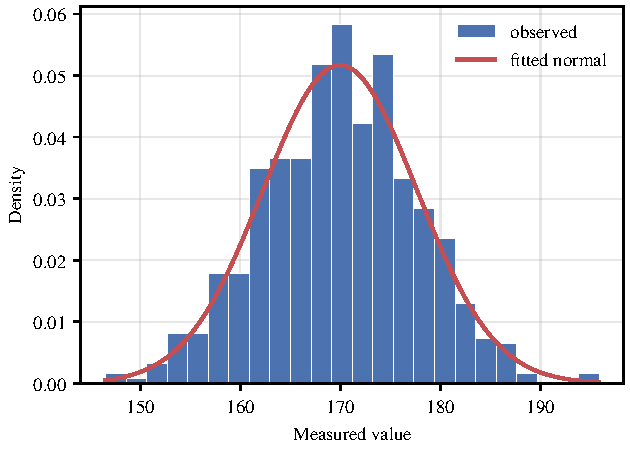
\includegraphics[width=0.7\linewidth]{figures/example-histogram.pdf}
  \caption[Distribution of a measured quantity]{Distribution of a measured
  quantity, with the fitted normal density drawn on top. Give the reader
  everything needed to interpret the figure without hunting through the body
  text: what was measured, how many observations, and what the curve is.}
  \label{fig:histogram}
\end{figure}

Figure~\ref{fig:histogram} is referenced by label, so its number survives being
moved to another chapter.

Several related panels belong in one float, each with its own sub-caption and
label:

\begin{figure}[htbp]
  \centering
  \begin{subfigure}{0.48\linewidth}
    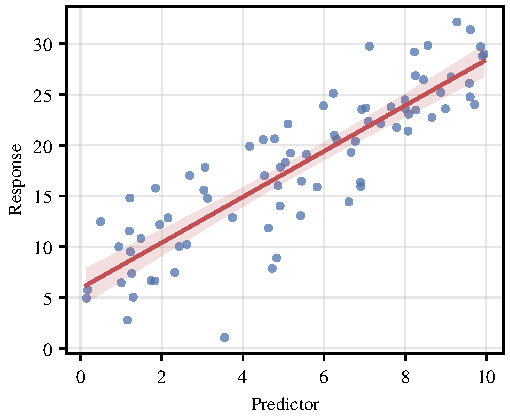
\includegraphics[width=\linewidth]{figures/example-scatter.pdf}
    \caption{Linear fit with a 95\% confidence band}
    \label{fig:scatter}
  \end{subfigure}
  \hfill
  \begin{subfigure}{0.48\linewidth}
    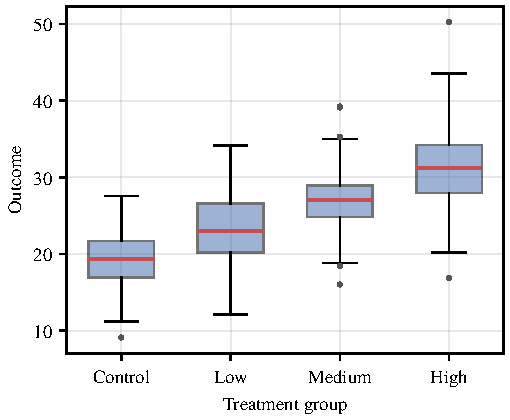
\includegraphics[width=\linewidth]{figures/example-boxplot.pdf}
    \caption{Distribution by treatment group}
    \label{fig:boxplot}
  \end{subfigure}

  \vspace{1em}

  \begin{subfigure}{0.48\linewidth}
    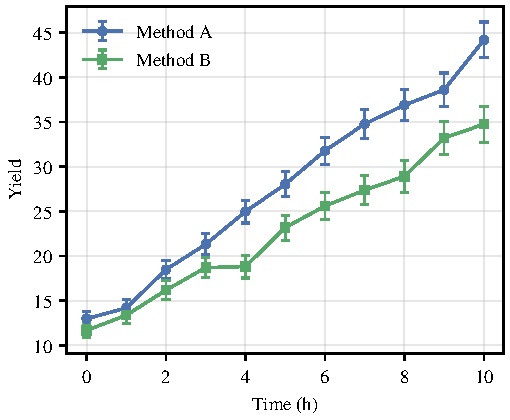
\includegraphics[width=\linewidth]{figures/example-errorbar.pdf}
    \caption{Two methods over time, with standard errors}
    \label{fig:errorbar}
  \end{subfigure}
  \caption[Three common ways of presenting a comparison]{Three common ways of
  presenting a comparison. Sub-figures are referenced individually, as in
  Figure~\ref{fig:scatter}, or as a group, as in Figure~\ref{fig:panels}.}
  \label{fig:panels}
\end{figure}

Vector PDFs keep their quality at any zoom level and are what plotting
libraries should be asked to emit. Bitmap formats are a last resort, and photos
belong in PNG or JPEG at a resolution high enough to survive printing.

\section{Tables}

\texttt{booktabs} gives tables the horizontal rules journals expect. Vertical
rules and double rules are deliberately hard to draw with it, because they make
tables harder to read.

\begin{table}[htbp]
  \centering
  \caption{Summary statistics by treatment group}
  \label{tab:summary}
  \begin{tabular}{lrrr}
    \toprule
    Group   & $n$ & Mean & Std.\ dev. \\
    \midrule
    Control &  90 & 19.8 & 4.1 \\
    Low     &  90 & 23.2 & 5.0 \\
    Medium  &  90 & 26.9 & 4.4 \\
    High    &  90 & 31.6 & 5.9 \\
    \bottomrule
  \end{tabular}
\end{table}

Table~\ref{tab:summary} sits above its data by convention: table captions go on
top, figure captions underneath. Note that the caption comes before the
tabular material in the source, and that a table wider than the text block
should be rotated or moved to an appendix rather than shrunk until it is
illegible.

\section{Source Code}

\texttt{minted} colours code through Pygments, which needs the compiler to run
with \verb|-shell-escape|. Overleaf enables this by default, and the local
build in this repository passes the flag for you.

\begin{minted}[fontsize=\small]{python}
def sample_variance(values):
    """Return the unbiased sample variance of a sequence of numbers."""
    n = len(values)
    if n < 2:
        raise ValueError("variance needs at least two observations")
    mean = sum(values) / n
    return sum((value - mean) ** 2 for value in values) / (n - 1)
\end{minted}

Short fragments read better inline: \mintinline{python}{sum(values) / n}.

\section{Citations}

\texttt{biblatex} manages citations, and \texttt{biber} processes the
bibliography. In \texttt{main.tex}, the configured
\mbox{\texttt{numeric-comp}} style compresses consecutive numbers into a range.

A plain citation looks like this~\cite{warren1890}. Several at once collapse
automatically~\cite{said1978,fisher1936,vaswani2017}. \texttt{biblatex} also
offers \verb|\parencite| for a parenthesised form~\parencite{surgeongeneral1964}
and \verb|\textcite| for one that reads as part of the sentence:
\textcite{geertz1973} makes this point directly.

The bibliography in \texttt{back/references.bib} carries one real, published
example of every entry type \texttt{biblatex} supports, so you can copy the
closest match rather than guessing which fields a type requires.

% !TeX root = ../main.tex

\chapter{Methods}\label{chap:methods}

\section{First Section}

Describe what you did in enough detail that somebody else could repeat it.

\lipsum[3][1-5]

\section{Second Section}

\lipsum[4][1-5]

% !TeX root = ../main.tex

\chapter{Results}\label{chap:results}

\section{First Section}

Report what you found, and only what you found. Save the interpretation for
Chapter~\ref{chap:discussion}.

\lipsum[5][1-5]

\section{Second Section}

\lipsum[6][1-5]

% !TeX root = ../main.tex

\chapter{Discussion}\label{chap:discussion}

\section{Interpretation}

Say what the results in Chapter~\ref{chap:results} mean, and how far the claims
in Chapter~\ref{chap:introduction} now stand.

\lipsum[7][1-5]

\section{Limitations}

State plainly what the work does not show. A committee trusts a thesis that
marks its own boundaries more than one that claims none.

\lipsum[8][1-4]

\section{Future Work}

\lipsum[9][1-4]


% 參考文獻
% References
\refmatter
% back/references.bib 為每種 biblatex 條目型別各準備一個範例。\nocite{*} 讓所有
% 條目都印出來，方便比對格式。開始寫論文時請刪掉這一行，否則未引用的條目也會列入。
% references.bib holds one example per biblatex entry type. \nocite{*} prints
% them all so the formatting can be compared. DELETE THIS LINE once you start
% writing, or uncited entries will show up in your bibliography.
\nocite{*}
\printbibliography

% 附錄
% Appendices
% !TeX root = ../main.tex

% \appendix{編號}{標題} — 編號與標題都要自己給。
% \appendix{LETTER}{TITLE} — both arguments are supplied by hand.
% 不需要附錄時，把 main.tex 裡對應的 \input 註解掉即可。
\appendix{A}{Supplementary Derivations}

\section{A Longer Derivation}

Material that would interrupt the argument in the body but that a careful
reader will want: full derivations, questionnaire text, or long parameter
tables.

\lipsum[10][1-4]

% !TeX root = ../main.tex

\appendix{B}{Supplementary Data}

\section{Additional Tables}

\lipsum[11][1-4]


\end{document}
